% !TEX root = ../main.tex

\section{Introduction}
Ethereum blockchain project\cite{Ref00} launched in 2014 by announcing Ether as its protocol-level cryptocurrency. It is ranked second in terms of market value after Bitcoin\footnote{CoinMarketCap - Ethereum currency - Accessed: 2019-02-11 \newline\url{https://coinmarketcap.com/currencies/ethereum/}} in 2019 and has the biggest development community to track enhancement and introduce new ideas\footnote{CoinDesk Crypto-Economics Explorer - Accessed: 2019-02-11 \newline\url{https://www.coindesk.com/data}}. Ethereum offers an ecosystem to implement any type of distributed applications (or DApps for short) on the blockchain that work together consistently. Tokens are essential part of this ecosystem that define common set of rules (known as API\footnote{Advanced Programming Interface}) for standardizing behavior of smart contracts\footnote{Or smart transaction: Types of transactions that execute as they are programmed by a scripting language (like Solidity or Viper)}. As a result, any ERC20-compliant application is aware of functionality of deployed tokens to employ them for exchanging, trading, transferring, etc. For example, shares of company X can be represented as ERC20 token. This makes it possible for other smart contracts to trade or exchange shares in form of digital assets. As shown in the below diagram, leveraging ERC20 tokens facilitate implementation of left side of the trading model on the blockchain:
\begin{figure}[H]
	\centering
	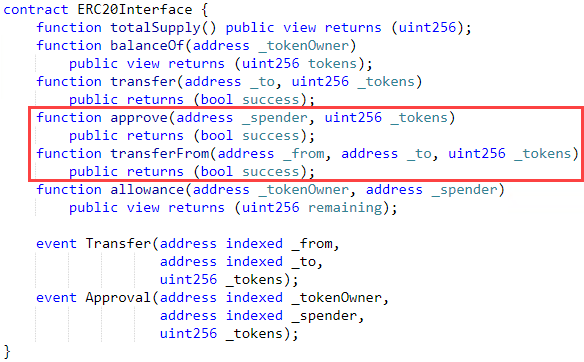
\includegraphics[width=1.0\linewidth]{figures/multiple_withdrawal_01.png}
	\caption{A blockchain trading model using ERC20 tokens.}
\end{figure}
Correspondingly, the right side of the model needs a financial asset which is equivalent to a fiat currency (like USD or CAD). Stablecoins\footnote{Types of digital assets that value of it will be stable over time and people be able to count on its value since it is pegging to something that has a stable value (like gold or USD).} provide this functionalities in blockchain and could also be represented as ERC20 token. Representing both share of company X and fiat currency as ERC20 tokens, give us two ERC20 tokens with different values to trade. This shows the importance of tokens in Ethereum ecosystem for digitizing tangible assets to digital equivalents. By using ERC20 tokens in the above example, we are able to migrate current centralized trading systems to the blockchain and taking advantage of a distributed trading system.

As mentioned before, ERC20 tokens are technically standardized version of smart contracts that could be vulnerable to security flaws. Some of these vulnerabilities have been already discovered and addressed by Ethereum community while there are few issue still open. In this paper, we analyze proposed community approaches and introduce new solution to one of these open issues that is known as "Multiple Withdrawal Attack". The issue is originally opened on GitHub\cite{Ref13} and raised as separate thread\cite{Ref07} for making it easy to follow. It is security issue in protocol-level and originating from definition of APIs in ERC20 standard for approving and transferring tokens. According to the standard specifications:
\begin{enumerate}
\item \textit{approve}\footnote{approve(address \_spender, uint256 \_tokens)} allows \textit{\_spender} to withdraw up to the \textit{\_value} amount of tokens from token pool of the approver. If this function is called again, it has to overwrites the current allowance with the new \textit{\_value}.
\item \textit{transferFrom}\footnote{transferFrom(address \_from, address \_to, uint256 \_tokens)} grants required rights to the spender (accounts, wallets or other smart contracts) for transferring \textit{\_value} amount of tokens from address \textit{\_from} to address \textit{\_to}.\newline
\end{enumerate}

Security issues at the protocol-level may impact already deployed ERC20 tokens and functionality of smart contracts based on them. In fact, using these functions (i.e., \textit{approve} and \textit{transferFrom}) in an undesirable situation could result in conditions that tokens being spent by another third party on behalf of the owner. Authors of the standard \cite{Ref08}, provided two sample codes from OpenZeppelin\cite{Ref10} and ConsenSys\cite{Ref11} as generic implementations. OpenZeppelin implementation uses two additional methods that initially proposed by MonolithDAO\cite{Ref12} and ConsenSys has not attempted to work around the issue. This issue is still open since October 2017 and several suggestions have been made that needs to be analyzed in term of compatibility with the standard and mitigation against the attack.
